% Chapter Template

\chapter{Methods} % Main chapter title

\label{Chapter2} % Change X to a consecutive number; for referencing this chapter elsewhere, use \ref{ChapterX}

%-------------------------------------------------------------------------------------
%	SECTION 1
%-------------------------------------------------------------------------------------

\section{Edge information helps to differentiate the pharynx from the intestine} \label{segMethod}

As described in \ref{limitationManual}, intestinal autofluorescence causes the static thresholding algorithm to perform insufficiently in separating the pharynx from the rest of the animal and the background. Histogram-based threshold detection such as Otsu's method also perform poorly when the histgrams are not bimodal, as is the case with bright intestinal autofluorescence.

To address these issues, a new segmentation algorithm was developed. This algorithm exploits \textit{edges}, sharp changes in brightness which are information-rich regions in images. The Sobel operator creates an image emphasizing edges by discretely differentiating the image in the vertical and horizontal directions (Figure \ref{fig:NewPipeline}). By thresholding the resultant image, using morphological operations to remove noise, and selecting the largest region, we isolate the pharynx from gut autofluorescence.

\begin{figure}[ht]
    \centering
    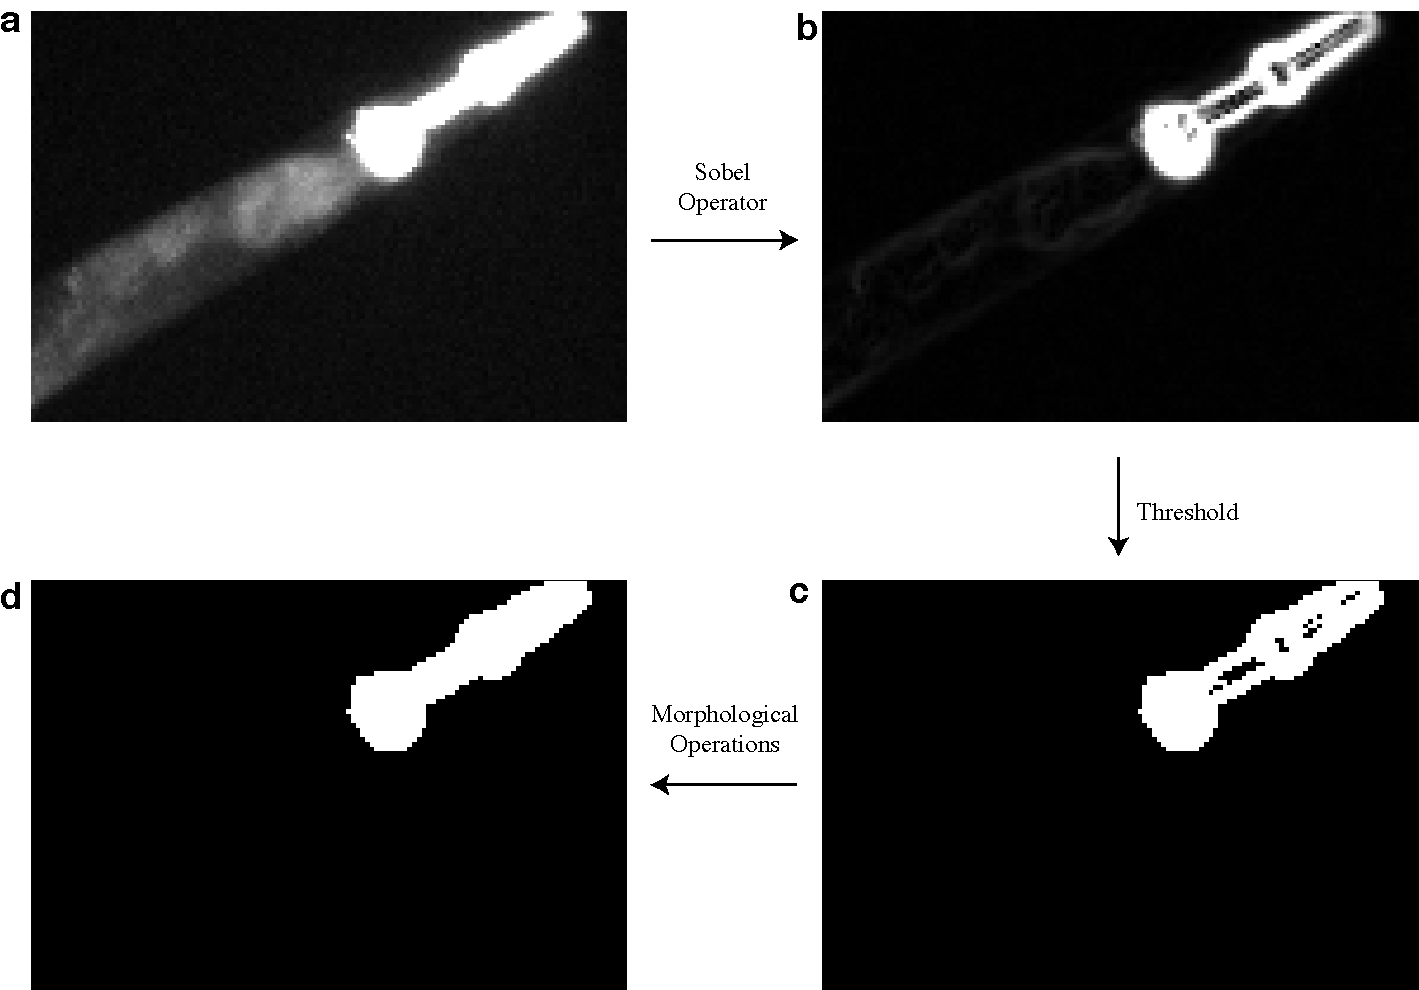
\includegraphics[scale=.40]{Figures/rendered_files/sobel}
    \decoRule
    \caption[Overview of the improved segmentation algorithm]{An overview of the improved segmentation algorithm. \textbf{a} The original image, displaying fluorescence of roGFP in the pharynx and the autofluorescence of the gut. \textbf{b} The resultant image after application of the sobel operator. \textbf{c} The resultant binary image after thresholding the edge-emphasized image. \textbf{d} The final segmented binary image, after performing morphological cleaning operations.}
    \label{fig:NewPipeline}
\end{figure}

For reasons described in \ref{TLMidlines}, an image taken with transmitted light must also be segmented. Even though the distribution of intensities in transmitted light images are very different from fluorescence images, this edge-based segmentation algorithm still performs robustly (Figure \ref{fig:TLSeg}). This highlights another benefit of the improved method: image brightness independence. If one particular genotype fluoresces dimly, an edge-based segmentation method still performs well, while the static threhsolding method requires the manual change of the threshold parameter.

\begin{figure}[ht]
    \centering
    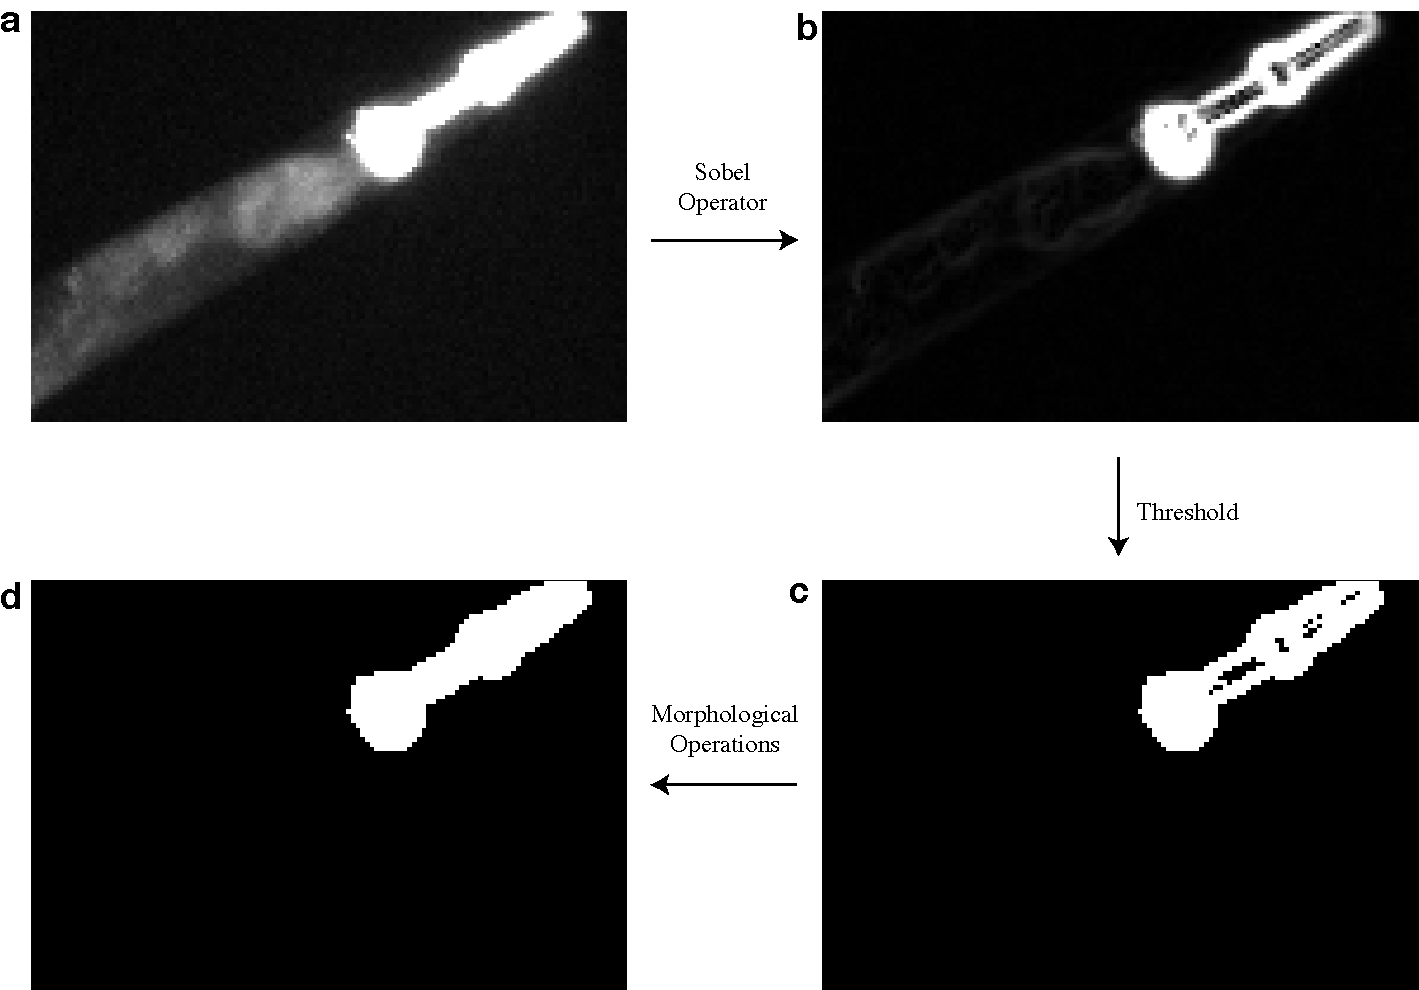
\includegraphics[scale=.40]{Figures/rendered_files/sobel}
    \decoRule
    \caption[Overview of the improved segmentation algorithm]{This should be an image of transmitted light before/after segmentation.}
    \label{fig:TLSeg}
\end{figure}

%-------------------------------------------------------------------------------------
%	SECTION 2
%-------------------------------------------------------------------------------------
\section{Flexible measurement boundaries allow for anterior-posterior movment} \label{channelSegmentation}

As described in \ref{limitations}, interframe movement is a large source of error.


The previous pipeline computes a single mask using the image taken at 410nm. This mask is then applied to both the 410nm and 470nm images. Measurements are taken of the masked image. Thus, if the animal pumps, measuremnt might start in the gut or halfway through the posterior bulb, depending on if the animal contracted during the first or second frame. If the animal contracts during the first frame and extends in the second, the mask will be too "short" and measurement in the second frame will start in the middle of the posterior bulb. If the animal is extended in the first frame and contracts in the second, the mask will be too "long" and measurement in the second frame will start in the gut.


The new approach is to create channel-specific masks for the purposes of drawing midlines. This allows the measurement boundaries to change on a frame-by-frame basis. That is, measurements always start at the posterior bulb and end at the tip.

%-------------------------------------------------------------------------------------
%	SECTION 3
%-------------------------------------------------------------------------------------
\section{Midlines} 
\subsection{A transmitted light image helps to anchor the midlines} \label{TLMidlines}

The previous centerline estimation algorithm takes as input an image of the pharynx aligned horizontally along its anterior posterior axis and works as follows (depicted in figure \ref{fig:oldMidline}).

\begin{figure}[ht]
    \centering
    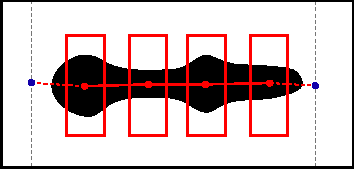
\includegraphics[scale=1.5]{Figures/rendered_files/old_midline_algorithm}
    \decoRule
    \caption[Previous centerline estimation algorithm]{Cartoon representation of the previous centerline estimation algorithm.}
    \label{fig:oldMidline}
\end{figure}

Boxes are drawn at specific static coordinates. The centroid of each shape is calculated (red points). Lines (solid) connect these points. The y-coordinates of the terminating points (blue) is determined via the point-slope method $y=mx+b$ where $m$ is the inverse of the slope of the neighboring line, $x$ is a fixed constant and $b$ is the y-coordinate of the neighboring point.

One problem 

The current centerline estimation algorithm is unstable around the posterior bulb. These instabilities must be manually corrected. Fundamentally, this problem arises because the  

\subsection{Dorsal-ventral movement of the tip is a problem} \label{frameSpecificMidlines}
We saw in \ref{channelSegmentation} a strategy to combat the major mode of inter-frame movement, contractions of the posterior bulb. However, there is another less common mode: dorsal-ventral movement of the tip. 


Again, frame-specific measurements are key to addressing this problem. Instead of using a single midline derived from the first frame, we calculate the midline independently in each frame. This frame-specific midline is then used to take profile measurements.

%-------------------------------------------------------------------------------------
%	SECTION 4
%-------------------------------------------------------------------------------------
\section{Channel Registration picks up the slack}

The frame-specific midline approach discussed in \ref{frameSpecificMidlines} introduces problems of its own. Specifically, the length of the measurement vector may be stretched nonlinearly due to differences in the arc length of each midline. That is, some sections of the intensity profile measured under these lines might be stretched while others are compressed. To approach these nonlinear stretches and compressions, we utilized a functionalized version of the dynamic time warping algorithm.

\todo[inline]{explanation of fda registration}